\chapter{Modellarchitektur und Ablauf}

Diese kleine Einleitung soll dem Nutzer helfen selbst die eigene Arbeit mit \LaTeX{} zu schreiben. Sie enthält zu den wichtigsten Themen Beispiele.


\section{2 Phasen der SER}

Für diese Arbeit lassen sich als Überschriften die Überschriften in verschiedenen Stufen verwenden.

\subsection{Verarbeitungseinheit (processing unit)}
\subsection{Klassifikator (classifier)}


\section{Aufbau der Modellarchitektur}


\begin{figure}[ht]
    \centering
    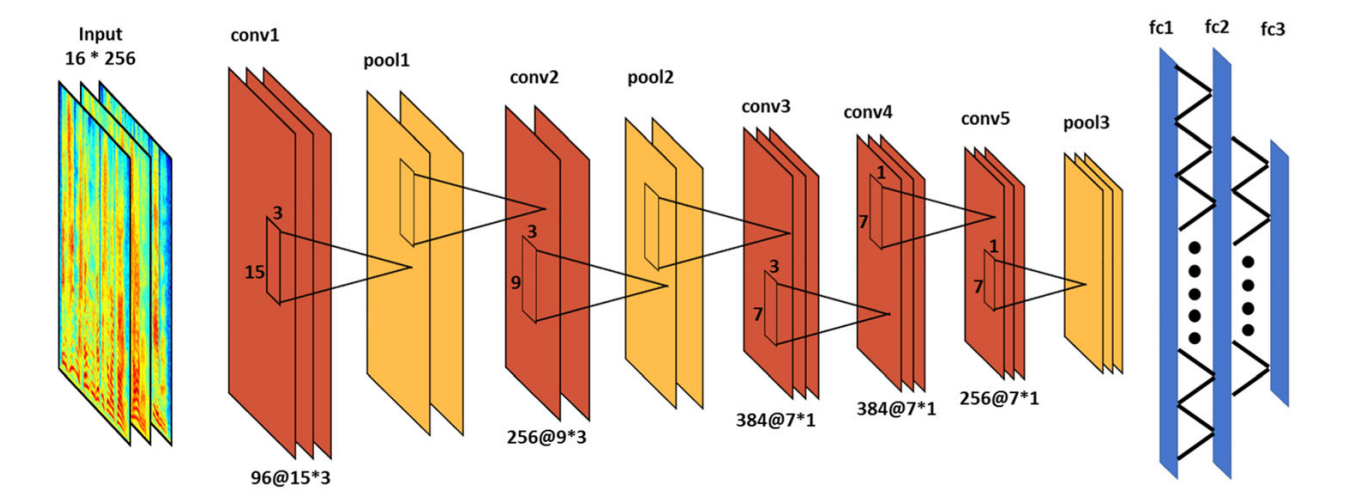
\includegraphics[width=1\textwidth]{images/conv}
    \caption{\label{architektur}CNN Architektur mit den unterschiedlichen Schichten \cite{badshah2019deep}}
\end{figure}

Mit Hilfe eines Labels kann man sich dann im Text auf diese Grafik (\ref{architektur}) beziehen. 



\section{Der Ablauf bei SER}

\begin{figure}[ht]
	\centering
	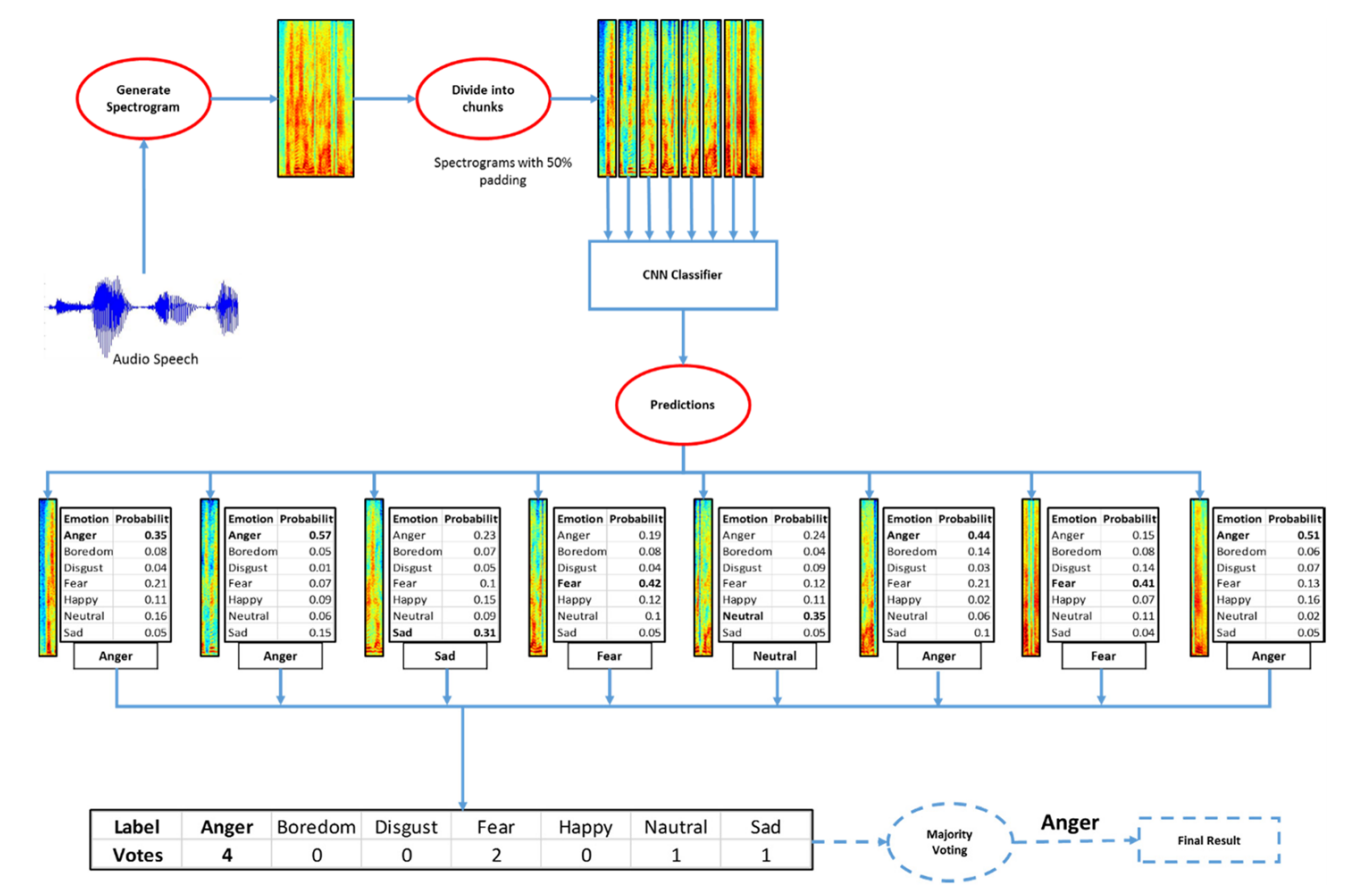
\includegraphics[width=1\textwidth]{images/ablauf}
	\caption{\label{ablauf}spezifischer Schema und Ablauf bei SER \cite{badshah2019deep}}
\end{figure}




